\section{B.~~Calibration of the readout circuit and energy coupling}
\makeatletter
\protected@edef\@currentlabel{B}
\label{sec:calibration}
\makeatother
\renewcommand\thefigure{\thesection B.\arabic{figure}} %To set the Fig numbering to A
\setcounter{figure}{0} 

\begin{comment}
This section is based on Supp. Mat. C in Fuchs et al.~\cite{Gravity}. 
The motion of the particle at the six resonance frequencies can be calibrated from flux to RMS motion by injecting an external current through the calibration transformer. The amount of current (or magnetic flux in the pick-up coil) injected is then directly quantified by the SQUID. The magnetic flux in the pick-up coil then exerts a force on the particle. By measuring the flux induced by the particle response, we find an absolute calibration of magnetic flux to motion. 

\begin{figure}[h]%
\centering
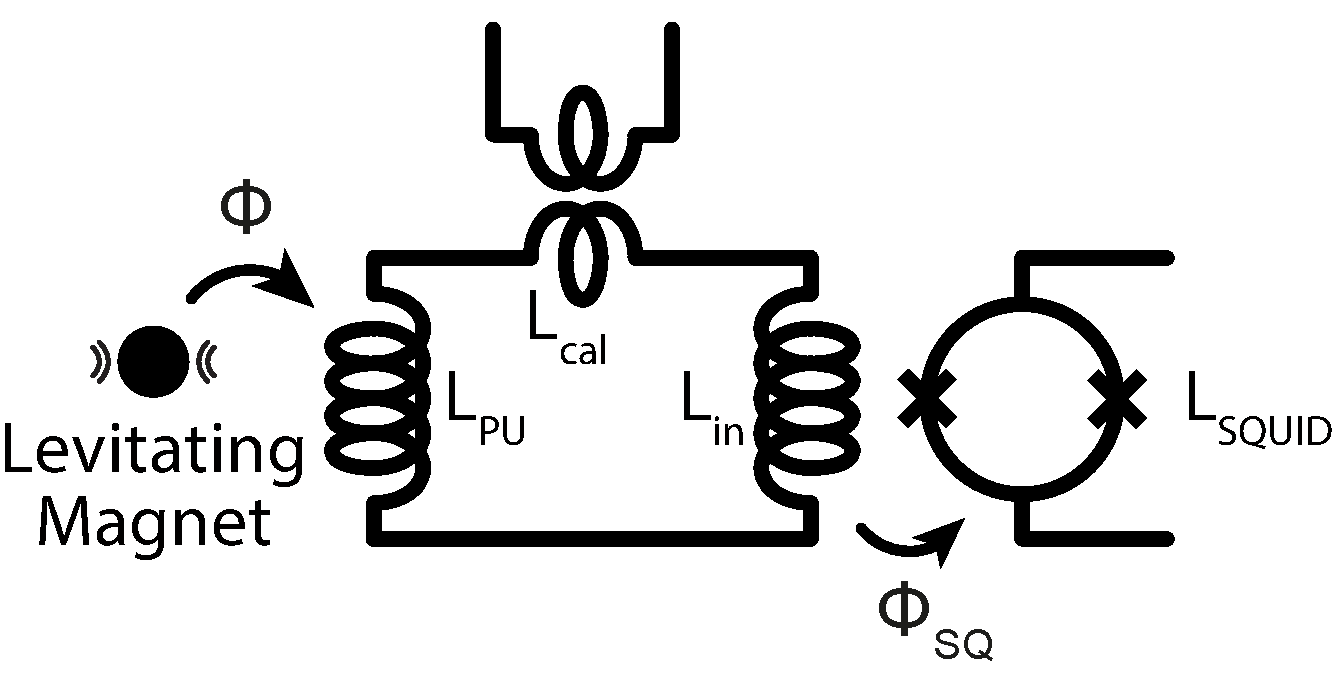
\includegraphics[width=\columnwidth]{5-Appendix/Figures/MLMP_circuit.pdf}
\caption{Schematic circuit of the single-stage readout circuit for the levitating magnet. The leviated magnet couples through a magnetic flux to the pick-up coil, with inductance $L_\text{PU}$, this flux is passed on to the SQUID via the input coil of the SQUID $L_\text{in}$ and additional flux can be added using the calibration transformer loop $L_\text{cal}$.}
\label{fig_app:readout_circuit}
\end{figure}

This calibration can be intuitively derived from the energy coupling ($\beta^2$). The energy coupling is defined as the fraction of the energies in two coupled oscillating systems, i.e. the amount of energy that couples from one system to the other. This energy coupling is similar to the quality factor of a single system, which is defined as the fraction of energy lost per cycle with respect to the total energy in the system, or equivalently, a measure for the damping of the system. Conversely, the quality factor provides a measure for the maximal energy stored in the resonator as a fraction of the input energy when driven at resonance for a time $T \gg \tau$, that is to say: the energy at which the fractional energy loss per cycle is equal to the energy put in each cycle by the resonant drive. 

For our system, with a mechanical resonator in the form of the levitating magnet, and a driving magnetic field coupled in through the calibration transformer and coupled to the magnet through the pick-up coil, we get 

\begin{equation}
    \beta^2 \equiv \frac{L_\text{total}I^2}{kx^2} 
\end{equation}

with $x$ any spatial coordinate and $L_\text{total} = L_\text{PU} + L_\text{in} + L_\text{cal}$ with the inductances as stated in Fig~\ref{fig_app:readout_circuit}. Going to the limit of infinitesimal displacement, and using $k =m\omega^2$, we obtain

\begin{equation}
    \beta^2 = \frac{\left(\frac{d\Phi}{dx}\right)^2}{L_\text{total}\cdot m\omega^2}
\end{equation}

from which it is evident that the energy coupling can be used to determine the absolute motion of the magnet from the flux measured in the SQUID.

To measure $\beta^2$, we further consider the motion of the resonator as a simple resonantly driven harmonic oscillator, with the \emph{Ansatz} $x(t) = A(t)e^{i\omega t};\ A(t) = \frac{F}{2 m \omega}\cdot t$, from which we obtain a driving force

\begin{equation}
    F_\text{driving} \left(= 2 m \zeta \omega_0 \frac{dx}{dt} = \gamma_\text{m} v \right)= \gamma_\text{m} \omega x .
\end{equation}

The quality factor ($Q_\text{drive}$) is equivalently defined as $Q_\text{drive} = \frac{1}{2\zeta}$, thus $\gamma_\text{m} = \frac{m\omega}{Q_\text{drive}}$.
In our calibration procedure, we inject a flux through the calibration transformer. This flux then results in a current through the detection circuit. This current is detected as a flux by the SQUID, with known $\frac{dI}{d\phi}$ calibration from the SQUID parameters. We refer to this current as the the crosstalk current $I_\text{crosstalk}$. This current also leads to a flux through the pick-up coil, which gives rise to a magnetic force on the particle of the form $F_\text{drive}=\alpha \cdot I_\text{crosstalk}$. Here, $\alpha$ is a coupling constant of units $\si{[N/A]}$ that contains a geometrical factor determined by both the relative positioning of the particle with respect to the pick-up coil, and the physical sizes of this coil and particle. As the particle is driven, the motion of the particle will in turn induce a current in the detection circuit. This induced current has the form $I_\text{induced}=\delta \cdot x$ where $\delta$ is a coupling constant with units $\si{[A/m]}$, which is by symmetry effected through the pick-up coil-particle geometry in the same way that $\alpha$ is.\\
Combining these results, and noting that for the steady state solution the driving force must be equal to the damping force

\begin{equation}
    \frac{I_\text{induced}}{I_\text{crosstalk}} =
    \frac{\delta\cdot x}{F_\text{drive}/\alpha} =
    \frac{\delta \cdot \alpha\cdot x}{\gamma_\text{m} \cdot \omega \cdot x} =
    Q \frac{\alpha\cdot\delta}{m\omega^2} = 
    Q \frac{\alpha\cdot\delta}{k} .
    \label{eq:I/I_1}
\end{equation}

Since some of our decay times are rather long, in our experiments we work with a $Q_\text{eff} = \pi fT_\text{drive}$, where $T_\text{drive}$ is the time during which the drive is applied. Whilst this is not the steady state, this discrepancy is fully absorbed in our definition of $Q_\text{eff}$:

\begin{equation}
    \frac{I_\text{induced}}{I_\text{crosstalk}} =
    \frac{\delta\cdot x}{F_\text{drive}/\alpha} =
    \frac{\delta \cdot \alpha\cdot x}{\gamma_\text{eff} \cdot \omega \cdot x} =
    Q_\text{eff} \frac{\alpha\cdot\delta}{m\omega^2} = 
    Q_\text{eff} \frac{\alpha\cdot\delta}{k} .
    \label{eq:I/I_2}
\end{equation}

From this derivation, we have found that the fraction of the currents in our detection circuit contains all the coupling constants in our system. In fact, looking at the units, we find
\begin{equation}
    \frac{\alpha\cdot\delta}{k} = 
    \frac{\si{\left[\frac{N}{A}\right]}\cdot\si{\left[\frac{A}{m}\right]}}{\si{\left[\frac{N}{m}\right]}}
\end{equation}
is dimensionless.

Furthermore, for small displacements in $x$, the flux change through the pick-up coil can be treated as linear. The resultant current in the detection circuit must then be $I_\text{induced} = \frac{d\Phi}{dx}\cdot x \cdot \frac{1}{L_\text{total}}$ or $\delta = \frac{d\Phi}{dx}\cdot \frac{1}{L_\text{total}} \hat{=} \si{\left[\frac{A}{m}\right]}$.

As noted before, $\delta$ contains the same geometric scaling as $\alpha$. From the symmetry, we recognise that $\alpha = \frac{d\Phi}{dx}$ ($\left[\text{Wb/m}\right]= \left[\text{N/A}\right]$). Combining these results, we find

\begin{equation}
    \frac{\alpha\cdot\delta}{k} = \frac{\left(\frac{d\Phi}{dx}\right)^2}{L_\text{total}\cdot m\omega^2} = \beta^2
\end{equation}

This final result gives us a procedure of how to measure $\beta^2$, or, conversely, the proportionality constant $\frac{d\Phi}{dx}$ that equates our measured flux to an absolute motion. The calibration measure is then found from 

\begin{equation}
    \frac{d\Phi}{dx} = \sqrt{L_\text{total}\cdot m\omega^2\cdot \beta^2} = \sqrt{L_\text{total}\cdot m\omega^2\cdot \frac{I_\text{induced}}{Q_\text{eff} \cdot I_\text{crosstalk}}}
\end{equation}

Noting that both $I_\text{induced}$ and $I_\text{crosstalk}$ are converted equally by the SQUID, the measured voltage can be inserted for the current through the detection circuit, which provides our sensitivity as 

\begin{equation}
    \frac{d\Phi}{dx} = \sqrt{L_\text{total}\cdot m\omega^2\cdot \frac{\Delta V_\text{drive}}{Q_\text{eff} \cdot V_\text{crosstalk}}}
\end{equation}

Here $\Phi$ is the flux through the pick-up coil. Since we detect this using the SQUID, we need to convert this value to the flux through the SQUID, which is done by dividing by the total inductance of the circuit and multiplying by the mutual inductance of the SQUID input loop and the SQUID loop ($M_\text{in,SQ}$). As a final step, this value can be related directly to the voltage measures made by taking the SQUID gain value as measured (${dV}/{d\Phi_\text{SQ}}$).  

The values for the inductances in $L_\text{total} = L_\text{PU}+L_\text{TP}+L_\text{in}+L_\text{cal}$ are: $L_\text{PU} = \SI{6.7e{-7}}{H}$ the inductance of the pick-up loop, $L_\text{TP} = \SI{1e{-7}}{H}$ the estimated inductance of the \SI{10}{cm} superconducting twisted-pair connecting the SQUID input to the pick-up coil, $L_\text{in} = \SI{1.8e{-6}}{H}$ the inductance of the input coil of the two-stage SQUID device, and $L_\text{cal} = \SI{2e{-9}}{H}$ the estimated inductance of the small calibration transformer coil. For the mutual inductance, the SQUID is calibrated to a value of $M_\text{in,SQ}^{-1} = \SI{0.5}{\micro A/\Phi_0}$. The SQUID voltage gain is measured as $dV/d\Phi_0 = \SI{0.43}{V/\Phi_0}$. These values, combined with measures of these ring-up's, gives us a value of $\frac{dV}{dx} = \SI{4.7}{{\frac{V}{\micro m}}}$ for mode 3 and $\frac{dV}{dx} = \SI{3.0}{{\frac{V}{\micro m}}}$ for mode 4, with a relative error of 8.5\%, which is dominated by the error in the mass.
\end{comment}

To calibrate the motion of the levitating magnet the method explained in Supp. Mat. C in Fuchs et al.~\cite{Gravity} is used. The main result of this derivation is equation S12 in this publication, giving the relationship between the measured voltage in the SQUID based measurement and the motional amplitude of the magnet, reading

\begin{equation}
    \frac{dV}{dx} = 
    \frac{dV}{d\Phi_\text{SQ}}\cdot\frac{d\Phi_\text{SQ}}{dI}\cdot\frac{dI}{d\Phi}\cdot\frac{d\Phi}{dx} =
    \frac{dV}{d\Phi_\text{SQ}} \cdot M_\text{in,SQ} \cdot \frac{1}{L_\text{total}}\cdot \frac{d\Phi}{dx}.
\end{equation}

Calculating these values for the two cooled modes gives us $\frac{dV}{dx} = \SI{4.7}{{\frac{V}{\micro m}}}$ for mode 3 and $\frac{dV}{dx} = \SI{3.0}{{\frac{V}{\micro m}}}$ for mode 4, with a relative error of 8.5\%, which is dominated by the error in the mass.

For a rotational mode the same method can be applied, and a value in units of \SI{}{[V/rad]} can be derived. To calculate a mode temperature this would result in a 
%in an integral over the angle, 
time average over the angle squared $ \left< \frac{1}{2} \kappa \theta^2 \right>_t$ in analogy to $ \left< \frac{1}{2} k x^2 \right>_t$, where $\kappa$ is the rotational stiffness, which calculates the energy in this rotational mode. If such a rotational mode is treated as a translational mode by accident and the mode temperature is calculated, the same result would be obtained as in the treatment of a rotational mode. 

%By means of conservation of energy the same energy is calculated in both cases and therefore the same mode temperature is obtained.



\begin{comment}
DU wil dit nog graag hebben voor later
\DU{wat doen we met de onzekerheid?}
\DU{Ik zou zeggen:\\
\begin{align}
    \frac{dV}{d\Phi_\text{SQ}} &\sim 1\% \\
    M_\text{in,SQ} &\sim 1\% \\
    L_\text{total} &\sim 2\% \\
    m &\sim 10\% \\
    \omega &\sim 1\% \\
    \Delta V_\text{drive} &\sim 1\% \\
    V_\text{crosstalk} &\sim 1\% \\
    Q_\text{eff} &\sim 5\% \\
\end{align}
Dan kom je uit op: 8.5\% waarbij de massa erg dominant is, als je die naar 5\% zet krijg je 5.9\% eruit, JWL: hebben we gekeken naar upper/lower bound, ik zou zeggen dat we eerder overschatten dan onderschatten, maar misschien zit ik mis
%https://www.wolframalpha.com/input?i=sqrt%280.01%5E2+%2B+0.01%5E2+%2B+0.02%5E2+%2B+1%2F2*%280.02%5E2%2B0.10%5E2%2B2*0.01%5E2+%2B+0.01%5E2+%2B+0.01%5E2%2B0.05%5E2%29%29
}
\DU{we doen 8.5\%}\\
\end{comment}
